\documentclass[norsk,a4paper]{article}\usepackage[]{graphicx}\usepackage[]{color}
%% maxwidth is the original width if it is less than linewidth
%% otherwise use linewidth (to make sure the graphics do not exceed the margin)
\makeatletter
\def\maxwidth{ %
  \ifdim\Gin@nat@width>\linewidth
    \linewidth
  \else
    \Gin@nat@width
  \fi
}
\makeatother

\definecolor{fgcolor}{rgb}{0.345, 0.345, 0.345}
\newcommand{\hlnum}[1]{\textcolor[rgb]{0.686,0.059,0.569}{#1}}%
\newcommand{\hlstr}[1]{\textcolor[rgb]{0.192,0.494,0.8}{#1}}%
\newcommand{\hlcom}[1]{\textcolor[rgb]{0.678,0.584,0.686}{\textit{#1}}}%
\newcommand{\hlopt}[1]{\textcolor[rgb]{0,0,0}{#1}}%
\newcommand{\hlstd}[1]{\textcolor[rgb]{0.345,0.345,0.345}{#1}}%
\newcommand{\hlkwa}[1]{\textcolor[rgb]{0.161,0.373,0.58}{\textbf{#1}}}%
\newcommand{\hlkwb}[1]{\textcolor[rgb]{0.69,0.353,0.396}{#1}}%
\newcommand{\hlkwc}[1]{\textcolor[rgb]{0.333,0.667,0.333}{#1}}%
\newcommand{\hlkwd}[1]{\textcolor[rgb]{0.737,0.353,0.396}{\textbf{#1}}}%

\usepackage{framed}
\makeatletter
\newenvironment{kframe}{%
 \def\at@end@of@kframe{}%
 \ifinner\ifhmode%
  \def\at@end@of@kframe{\end{minipage}}%
  \begin{minipage}{\columnwidth}%
 \fi\fi%
 \def\FrameCommand##1{\hskip\@totalleftmargin \hskip-\fboxsep
 \colorbox{shadecolor}{##1}\hskip-\fboxsep
     % There is no \\@totalrightmargin, so:
     \hskip-\linewidth \hskip-\@totalleftmargin \hskip\columnwidth}%
 \MakeFramed {\advance\hsize-\width
   \@totalleftmargin\z@ \linewidth\hsize
   \@setminipage}}%
 {\par\unskip\endMakeFramed%
 \at@end@of@kframe}
\makeatother

\definecolor{shadecolor}{rgb}{.97, .97, .97}
\definecolor{messagecolor}{rgb}{0, 0, 0}
\definecolor{warningcolor}{rgb}{1, 0, 1}
\definecolor{errorcolor}{rgb}{1, 0, 0}
\newenvironment{knitrout}{}{} % an empty environment to be redefined in TeX

\usepackage{alltt}
\usepackage[norsk]{babel}
\usepackage[utf8x]{inputenc}
\usepackage{subfig}
\usepackage{pdfpages}
\usepackage{booktabs}
\usepackage{caption}
\usepackage{amssymb}

\title{Testrapport for NGER}
\author{Yusman Kamaleri \& Kevin Thon (SKDE)}

\renewcommand\thempfootnote{\fnsymbol{mpfootnote}}
\def\labelitemi{$\bullet$}
\def\labelitemii{--}
\def\labelitemiii{$\ast$}
\def\labelitemiv{$\cdot$}

%setter grå skrift fremfort sort
\usepackage{xcolor}
\usepackage{graphicx}
% \definecolor{SKDE}{rgb}{0,0.32,0.61}
% \definecolor{lysblaa}{rgb}{0.27,0.51,0.71}
% \definecolor{moerkblaa}{rgb}{0.0,0.0,0.47}
% \definecolor{lysgraa}{rgb}{0.8,0.8,0.8}
% \definecolor{middelsgraa}{rgb}{0.5,0.5,0.5}
\definecolor{moerkgraa}{rgb}{0.25,0.25,0.25}
\color{moerkgraa}
\IfFileExists{upquote.sty}{\usepackage{upquote}}{}
\begin{document}
% \thispagestyle{empty}
% \includepdf[fitpaper]{../ForsideV1logo.pdf}
% \thispagestyle{empty}
% \cleardoublepage
% \setcounter{page}{1}

\addtolength{\hoffset}{-0.5cm}
\addtolength{\textwidth}{1cm}
\addtolength{\voffset}{-1cm}
\addtolength{\textheight}{2cm}

\maketitle

\tableofcontents
\newpage

\listoffigures
\listoftables

\clearpage



%'
%' <<'TestDebug', results='asis', echo=FALSE, eval=T, warning=TRUE>>=
%' libkat <- 'C:/SVN/jasper/Rlib/trunk/'
%'
%' figstr <- 0.58
%' source("C:/SVN/jasper/nger/trunk/NGERAntallRegPrAvd.R", encoding = "UTF-8")
%' source("C:/SVN/jasper/nger/trunk/NGERFigAndeler.R", encoding = "UTF-8")
%'
%' datoFra='2013-01-01'
%' datoTil=Sys.Date()
%' @

% \addtolength{\hoffset}{-1.5cm}

\section{Registrerende avdelinger}

% latex table generated in R 3.2.3 by xtable 1.8-2 package
% Thu Feb 18 13:46:45 2016
\begin{table}[ht]
\centering
\begin{tabular}{lrrr}
  \hline
 & 2014 & 2015 & 2016 \\ 
  \hline
Finnmarkssykehuset HF & 73 & 93 & 1 \\ 
  Helgelandssykehuset & 71 & 120 & 10 \\ 
  Helse Bergen HF & 366 & 347 & 22 \\ 
  Helse Førde HF & 73 & 39 & 1 \\ 
  Helse Fonna HF & 0 & 261 & 19 \\ 
  Helse Møre og Romsdal HF & 222 & 192 & 0 \\ 
  Helse Stavanger HF & 201 & 127 & 6 \\ 
  Nordlandssykehuset HF & 156 & 198 & 6 \\ 
  Oslo universitetssykehus HF & 808 & 726 & 70 \\ 
  Sørlandet sykehus HF & 30 & 17 & 0 \\ 
  St. Olavs Hospital HF & 2 & 1 & 0 \\ 
  Sykehuset i Vestfold HF & 342 & 503 & 50 \\ 
  Sykehuset Innlandet HF & 360 & 319 & 32 \\ 
  Universitetssykehuset Nord-Norge HF & 2 & 21 & 14 \\ 
  Vestre Viken HF & 277 & 220 & 22 \\ 
   \hline
\end{tabular}
\caption{Liste over avdelinger som registrerer pasienter i NoRGast.} 
\label{tab:RegistrenrendeAvd}
\end{table}





\begin{figure}[ht]
\centering
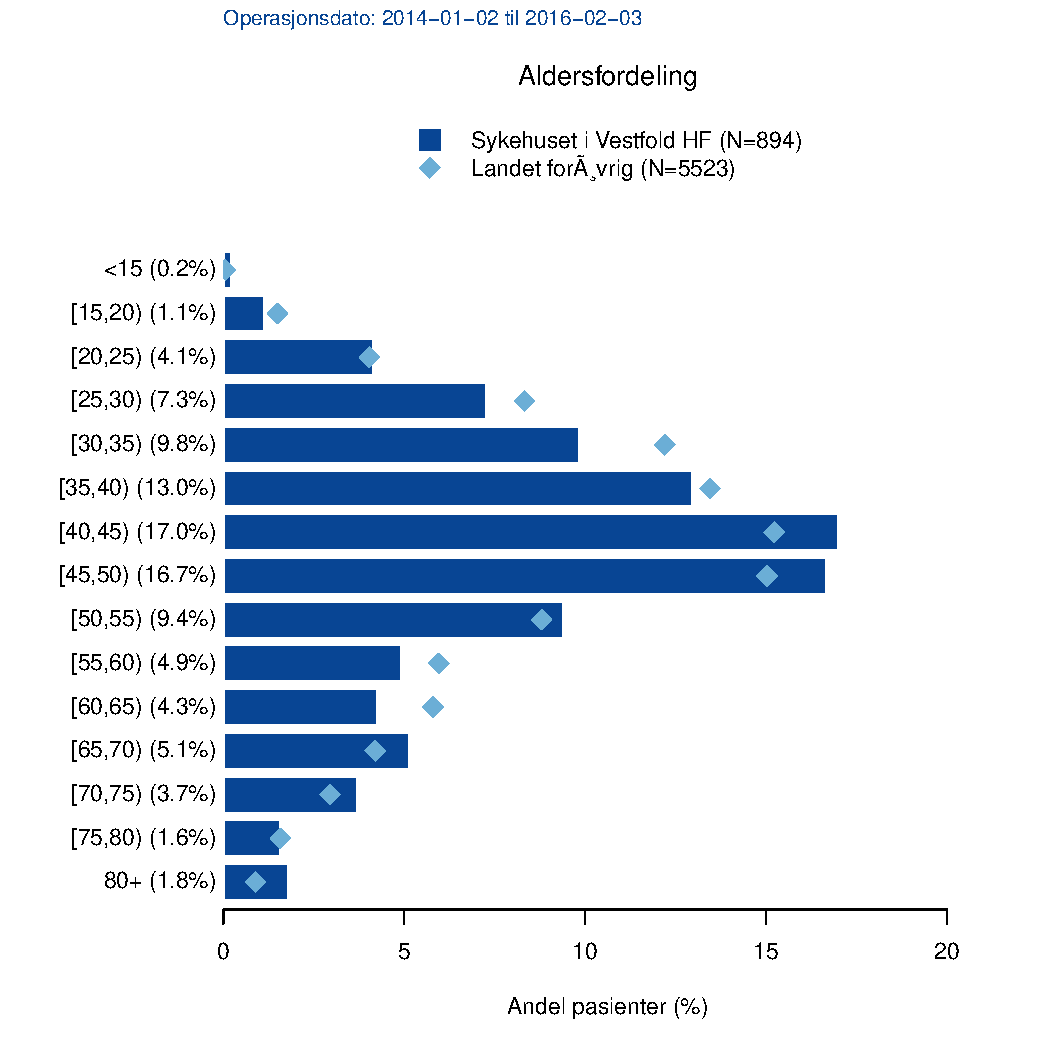
\includegraphics[width=0.58\textwidth]{test.pdf}
\caption{testfigur for nger}
\end{figure}


\end{document}
